Wydarzenia od zawsze stanowiły integralną część życia społecznego. Początkowo jedyną formą informowania o odbywających się wydarzeniach była forma  ustna. Wraz z rozwojem cywilizacji ludzkość zaczęła posługiwać się pismem, co umożliwiło zapisywanie informacji o wydarzeniach i sporządzanie listy uczestników. Umożliwiło to także precyzyjne planowanie oraz dokładne dokumentowanie uroczystości przez osoby wykształcone, posługujące się pismem.

Kluczowym momentem w rozwoju wydarzeń było wynalezienie druku w 1450 roku przez Jana Gutenberga. Pozwoliło to na zwiększenie ilości materiałów informacyjnych oraz ich dystrybucję i archiwizację. Wraz z rozwojem technologii druku, w 1609 roku w Strasburgu powstała pierwsza gazeta, co przyczyniło się do tworzenia powierzchni reklamowych dla wszelkich wydarzeń oraz zwiększyło dostęp do informacji i zainteresowanie społeczeństwa. \autocite{gazeta}

Rewolucja przemysłowa na przełomie XVIII i XIX wieku przyczyniła się do znaczących zmian w zakresie zarządzania i organizacji wydarzeń. Dostęp informacji dla społeczeństwa został znacząco zwiększony, co przyczyniło się do rozwoju mediów oraz reklamy. Masowo drukowane ulotki i gazety znacznie zwiększyły zasięg informacji o wydarzeniach, co przyczyniło się do zwiększenia liczby uczestników. Obecność afiszu teatralnego z 1799 roku (\autoref{rys:afisz}) stanowi doskonały przykład, ilustrujący, jak technologiczne innowacje wpłynęły na zwiększenie zasięgu informacji o wydarzeniach i sprzyjały wzrostowi liczby uczestników, tworząc dynamiczne środowisko kulturalne i społeczne.

\begin{figure} [H]
    \begin{center}
    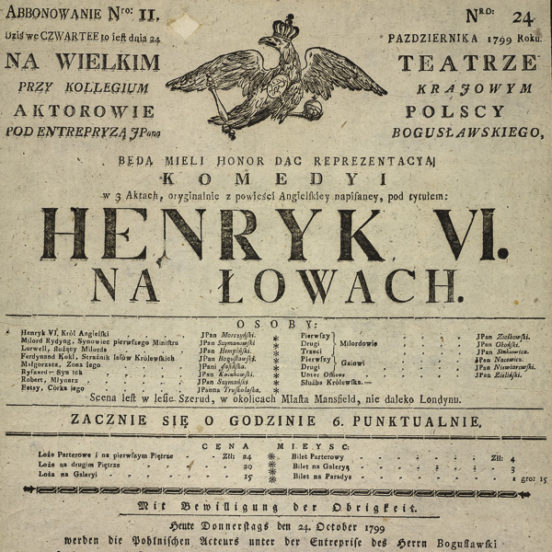
\includegraphics[scale=0.20]{imgs/afisz.jpg}
    \end{center}
    \caption{Afisz teatralny z 1799 roku \autocite{polona}}
    \label{rys:afisz}
    \end{figure}

W końcówce XX wieku wraz z pojawieniem się ogólnodostępnych technologii komputerowych pojawiły się pierwsze systemy informatyczne wspomagające organizację wydarzeń. Wraz z rozwojem Internetu i technologii mobilnych, systemy informatyczne stały się coraz bardziej dostępne i popularne, co umożliwiło ich wykorzystanie w organizacji wydarzeń np. poprzez użycie kodów QR do sprawdzania obecności na wydarzeniu. Obecnie systemy informatyczne stanowią integralną część organizacji wydarzeń, a ich rozwój jest dynamiczny i nieustanny.